%!TEX root = ../D5.4.tex

\section{Experimental Design}
%
In this experiment the iCub is torque controlled. The control algorithm relies on the inverse-dynamics 
control scheme that was presented in \cite{NoriTrav2015}. Human dynamics and kinematics are monitored by 
whole-body distributed IMU sensors and contact forces at the feet are measured with two force platforms.
%
%%%%%%%%%%%%%%%%%%%%%%%%%%%%%%%%%%%%%%%%%%%%%%%%%%%%%%%%%%%%%%%%%%%%%%%%%%%%%%%%%%%%%%%%%%%%%%%%
\subsection{Human wearable sensors for dynamic estimation}
 Human kinematics data were acquired by using a full-body wearable lycra suit provided by Xsens Technologies.  
The wearable suit is composed of 17 wired trackers, (i.e., inertial sensor units-IMUs including an
 accelerometer, a gyroscope and a magnetometer). The suit has signal transmitters that send
  measurements to the acquisition unit through a wireless receiver which collects data at a
   frequency of \unit{240}{\hertz}. The human subject performed the required
    task standing with the
   feet on two standard force platforms AMTI OR6 mounted on the ground, while interacting 
   with the robot.
	  Each platform acquired a wrench sample at a frequency of
	   \unit{1}{\kilo\hertz} by using AMTI acquisition units. 
%
\begin{figure}
  \centering
    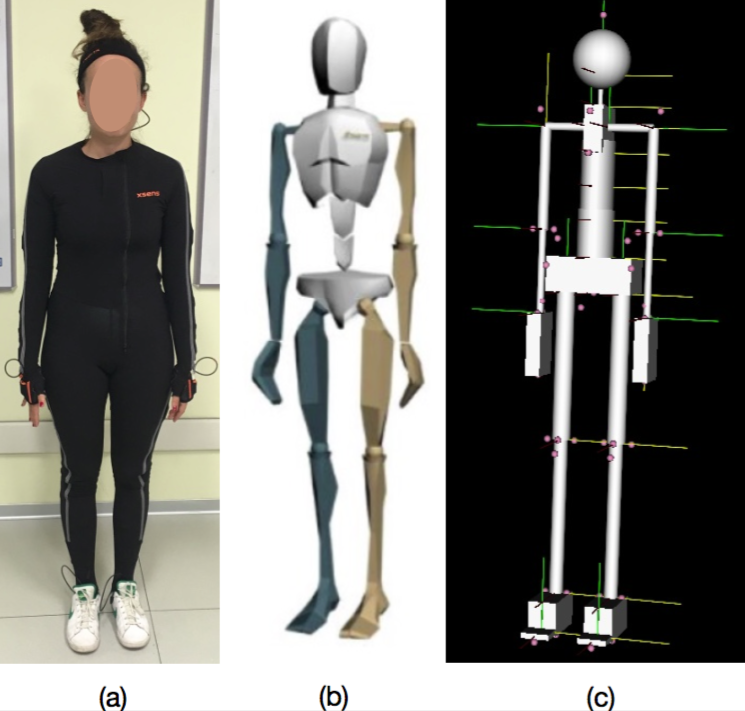
\includegraphics[width=0.9\columnwidth]{figs/humanModels}
  \caption{(a) Subject with the motion capture suit. (b) The Xsens MVN model. (c) Model reconstructed in OpenSim by using virtual markers from Xsens acquisition.}
 \label{fig:human_models}
\end{figure}
%
%%%%%%%%%%%%%%%%%%%%%%%%%%%%%%%%%%%%%%%%%%%%%%%%%%%%%%%%%%%%%%%%%%%%%%%%%%%%%%%%%%%%%%%%%%%%%%%%
\subsection{Robot sensors for dynamic estimation}
Experiments were conducted on the iCub \cite{Metta2010}, a full-body humanoid
robot (Fig. \ref{fig:iCub_couple}a) with 53-DoFs: 6 in the head, 16 in each arm, 3 in the
 torso and 6 in each leg. The iCub is endowed with whole-body distributed force/torque sensors,
  accelerometers, gyroscopes and tactile sensors. Specifically, the limbs are equipped with six
   force/torque sensors placed in the upper arms, in the upper legs and in the ankles 
   (Fig. \ref{fig:iCub_couple}b). Internal joint torques and external wrenches are estimated
    through an online whole-body estimation algorithm \cite{Nori2015icub}. Measurements for the
    wrenches exchanged between the robot and the human are obtained thanks to it.  Robot data
	 were collected at a frequency of \unit{100}{\hertz}.
%
\begin{figure}
  \centering
    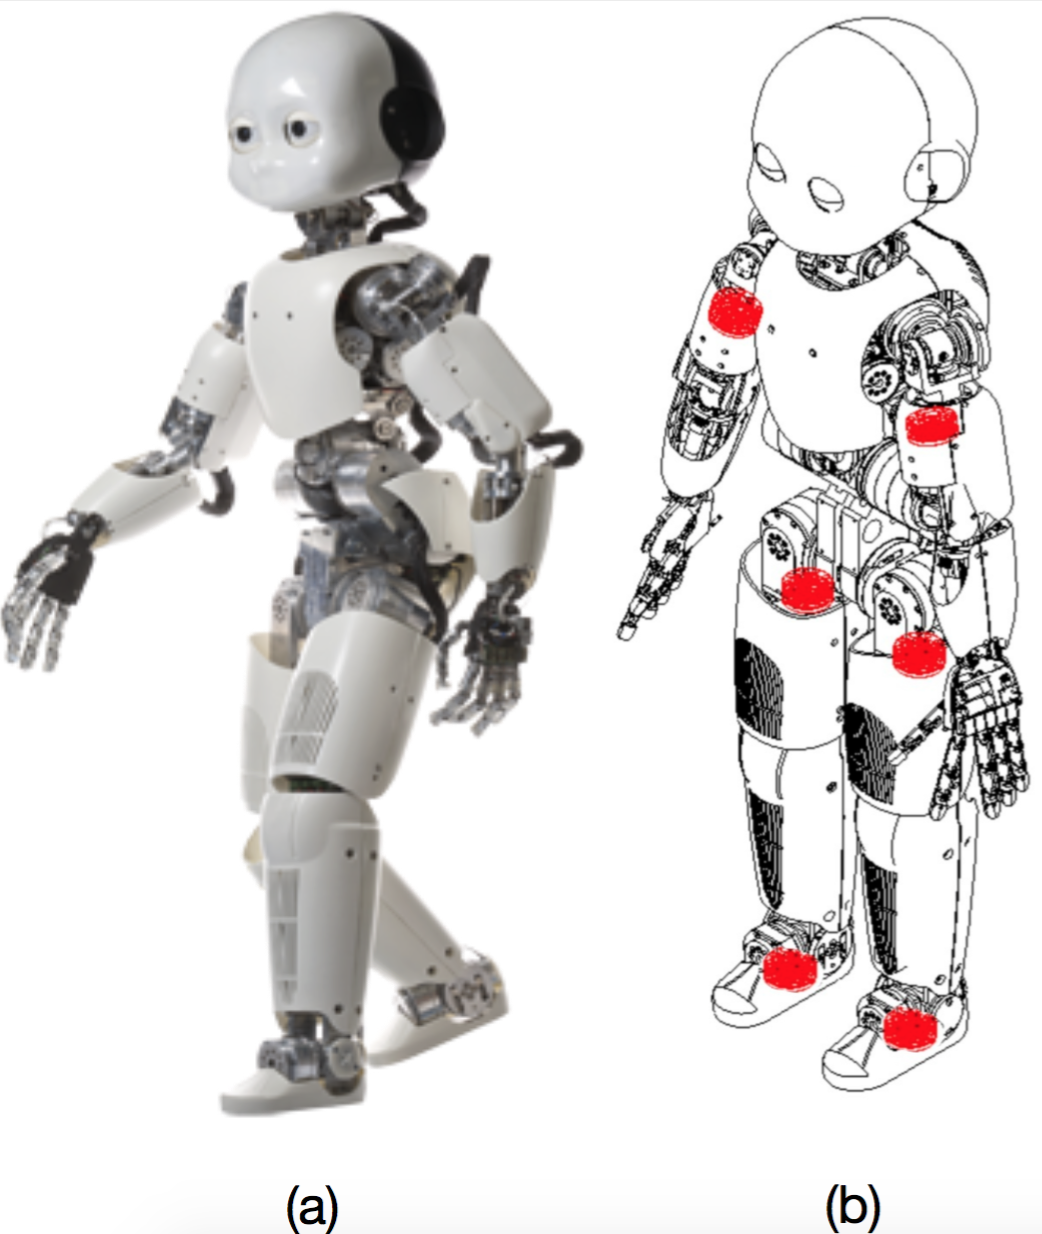
\includegraphics[width=0.55\columnwidth]{figs/iCub_couple}
  \caption{(a) The humanoid iCub. (b) Model of the iCub with the force/torque 
  sensors embedded in the limbs structure.}
  \label{fig:iCub_couple}
\end{figure}

\begin{figure}
  \centering
    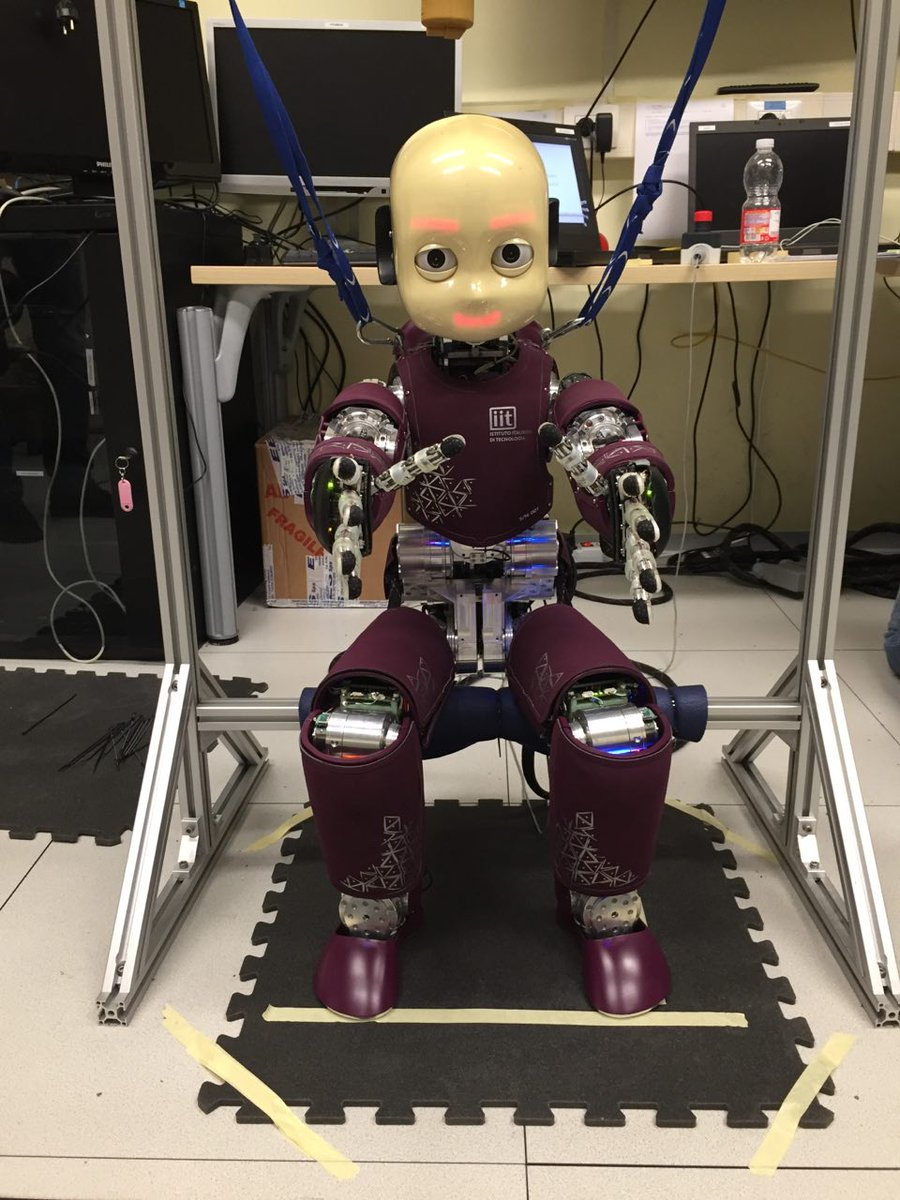
\includegraphics[width=0.45\columnwidth]{figs/iCubStool1} \hspace{1cm}
    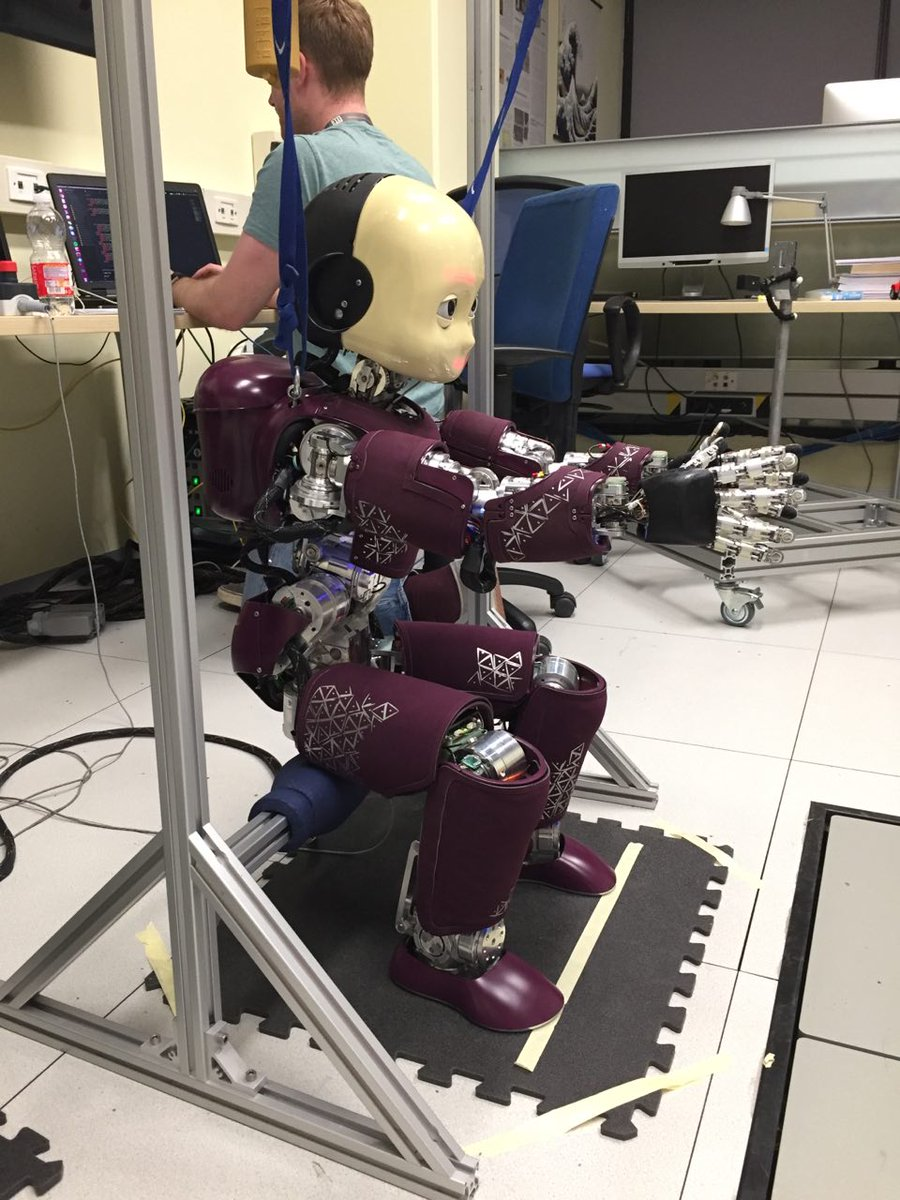
\includegraphics[width=0.45\columnwidth]{figs/iCubStool2}
  \caption{The iCub is initially seating on a stool while keeping the feet on the ground. }
  \label{fig:iCubStool}
\end{figure}
%
%%%%%%%%%%%%%%%%%%%%%%%%%%%%%%%%%%%%%%%%%%%%%%%%%%%%%%%%%%%%%%%%%%%%%%%%%%%%%%%%%%%%%%%%%%%%%%%%
\subsection{Procedure protocol}
The interacting subject (e.g. caregiver) wears the suit (Fig. \ref{fig:human_models}a) and stands on the 
two force plates by positioning each foot on a platform. The robot 
is located in front of the subject, facing him and  seating on a stool.
It maintains balance with the whole-body inverse dynamics approach described in \cite{NoriTrav2015}.
During the experiment, human and robot interact by exchanging forces at predefined locations. 
At this stage, the interaction was chosen to occur at the iCub forearm to avoid mechanical failures
due to the fragility of the iCub hands  (as shown in Fig. \ref{fig:interaction_lateral&top}a).
Also the relative human-robot distance
is fixed by requiring the human subject to place the feet at specific locations on a printed paper
which sketches the experiment layout and is placed on the floor (Fig. \ref{fig:interaction_lateral&top}b). 

The basic control strategy for the standing motion relies on whole-body inverse dynamics.
The controller is implemented in Simulink\footnote{\url{https://github.com/robotology-playground/WBI-Toolbox-controllers}}
and has been successfully tested in 
simulation (see Fig.~\ref{fig:iCubSimStanding}) and on the real robot (see Fig.~\ref{fig:iCubStanding}).
In its current version the controller performs the standing up motion without the help
of the caregiver, i.e. without any physical human-robot interaction. 

  
%
\begin{figure}[ht]
  \centering
    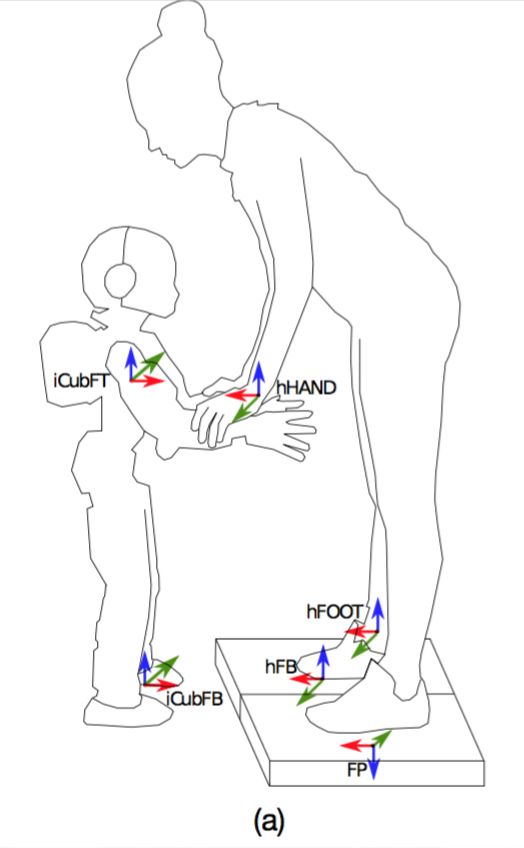
\includegraphics[height=6cm]{figs/interaction_lateralAndTop2} \hspace{1cm}
    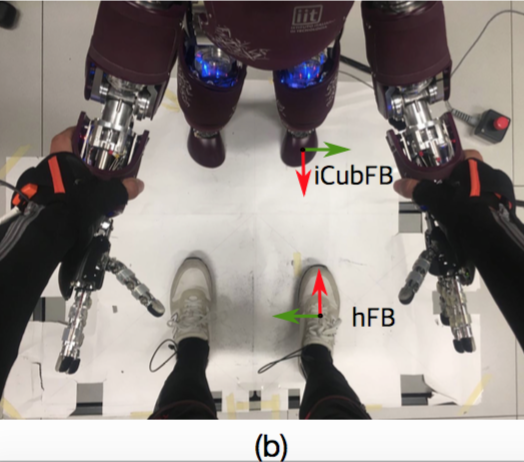
\includegraphics[height=6cm]{figs/interaction_lateralAndTop}
          \caption{(a) The figure shows the
		  reference frames for the force/torque sensor of the robot (iCubFT), the robot fixed
		   base (iCubFB), the force plate (FP), the human fixed base (hFB), the human foot and
		    hand (hFOOT, hHAND) respectively. (b) Top view for the feet position layout.}
			\label{fig:interaction_lateral&top}
\end{figure}

\begin{figure}
  \centering
    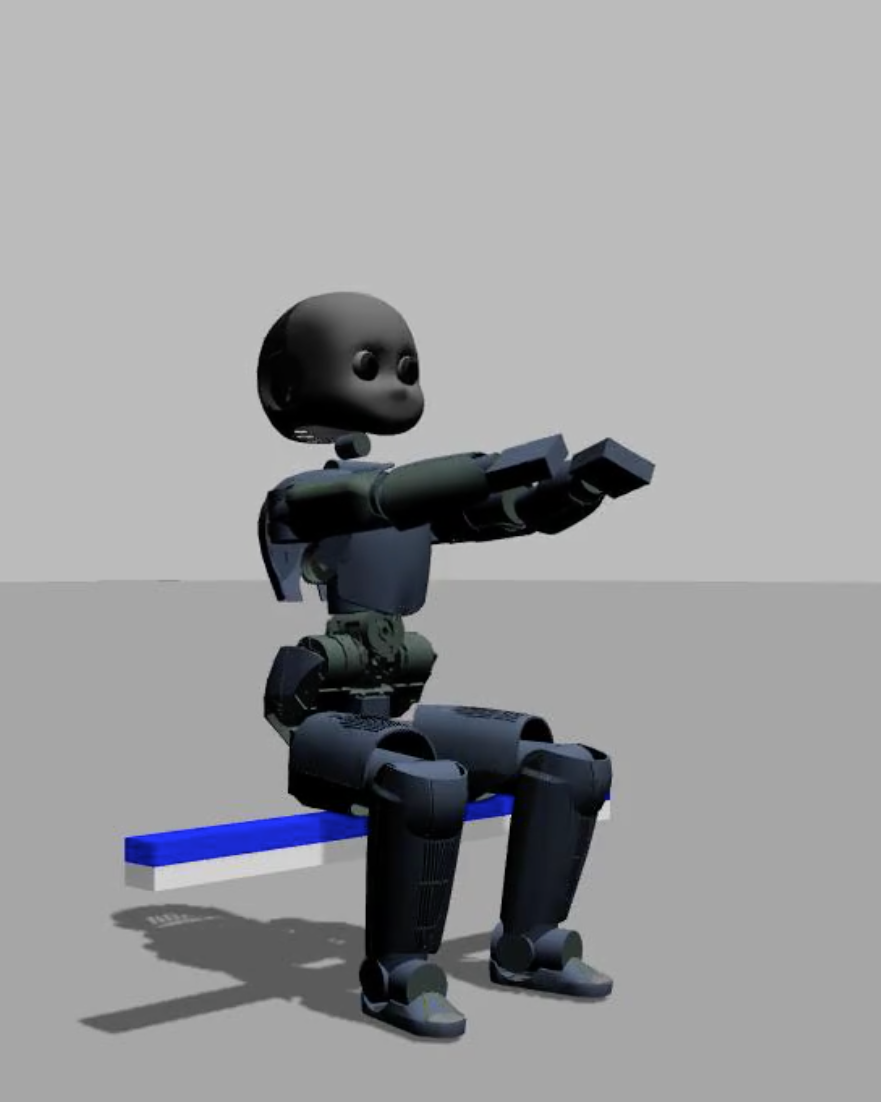
\includegraphics[width=0.2\columnwidth]{figs/standingSim_1} \hspace{1cm}
    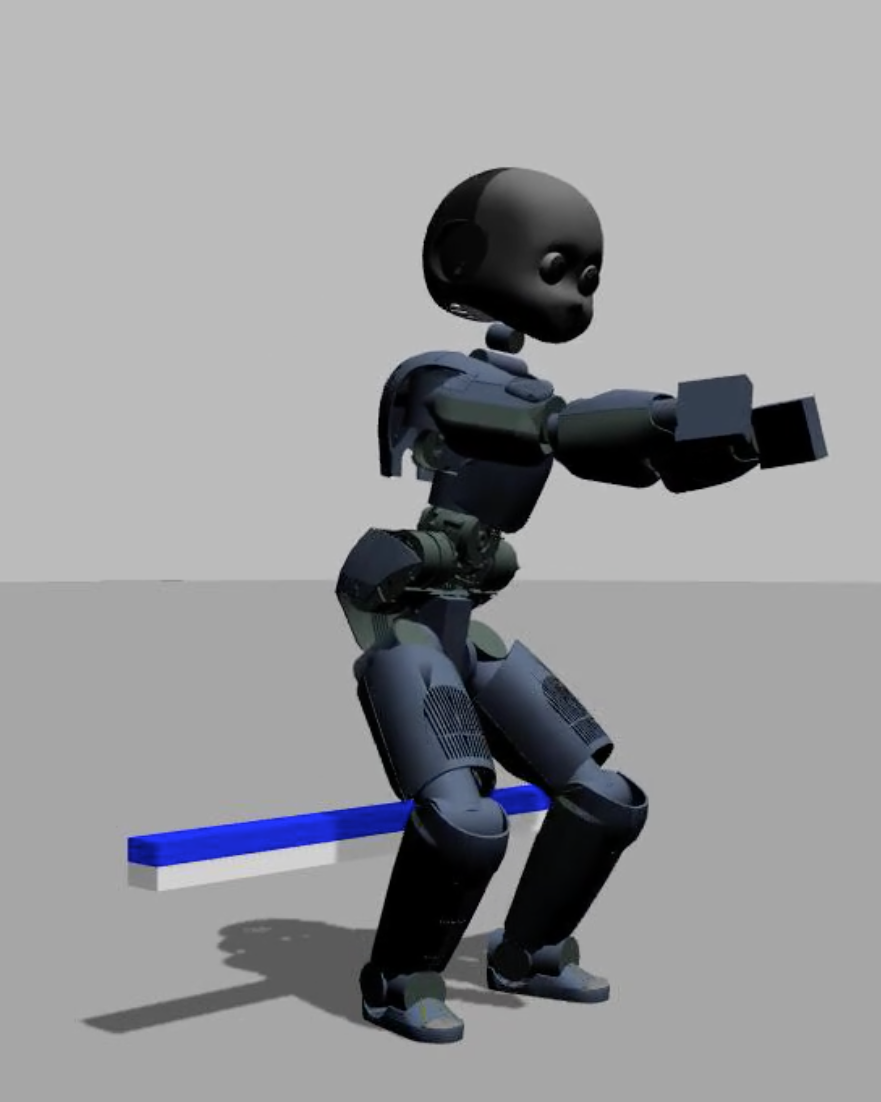
\includegraphics[width=0.2\columnwidth]{figs/standingSim_2} \hspace{1cm}
    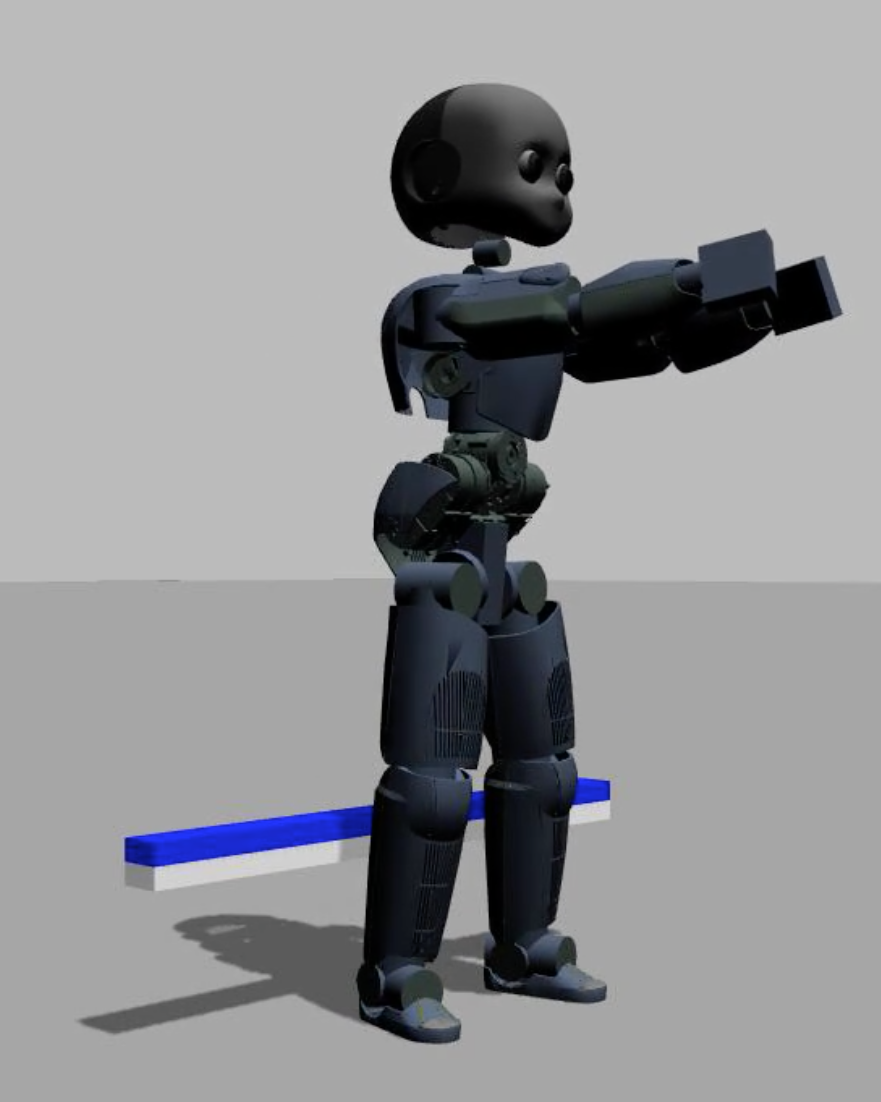
\includegraphics[width=0.20\columnwidth]{figs/standingSim_3}
  \caption{The iCub simulated standing motion without external support from a caregiver. }
  \label{fig:iCubSimStanding}
\end{figure}

\begin{figure}
  \centering
    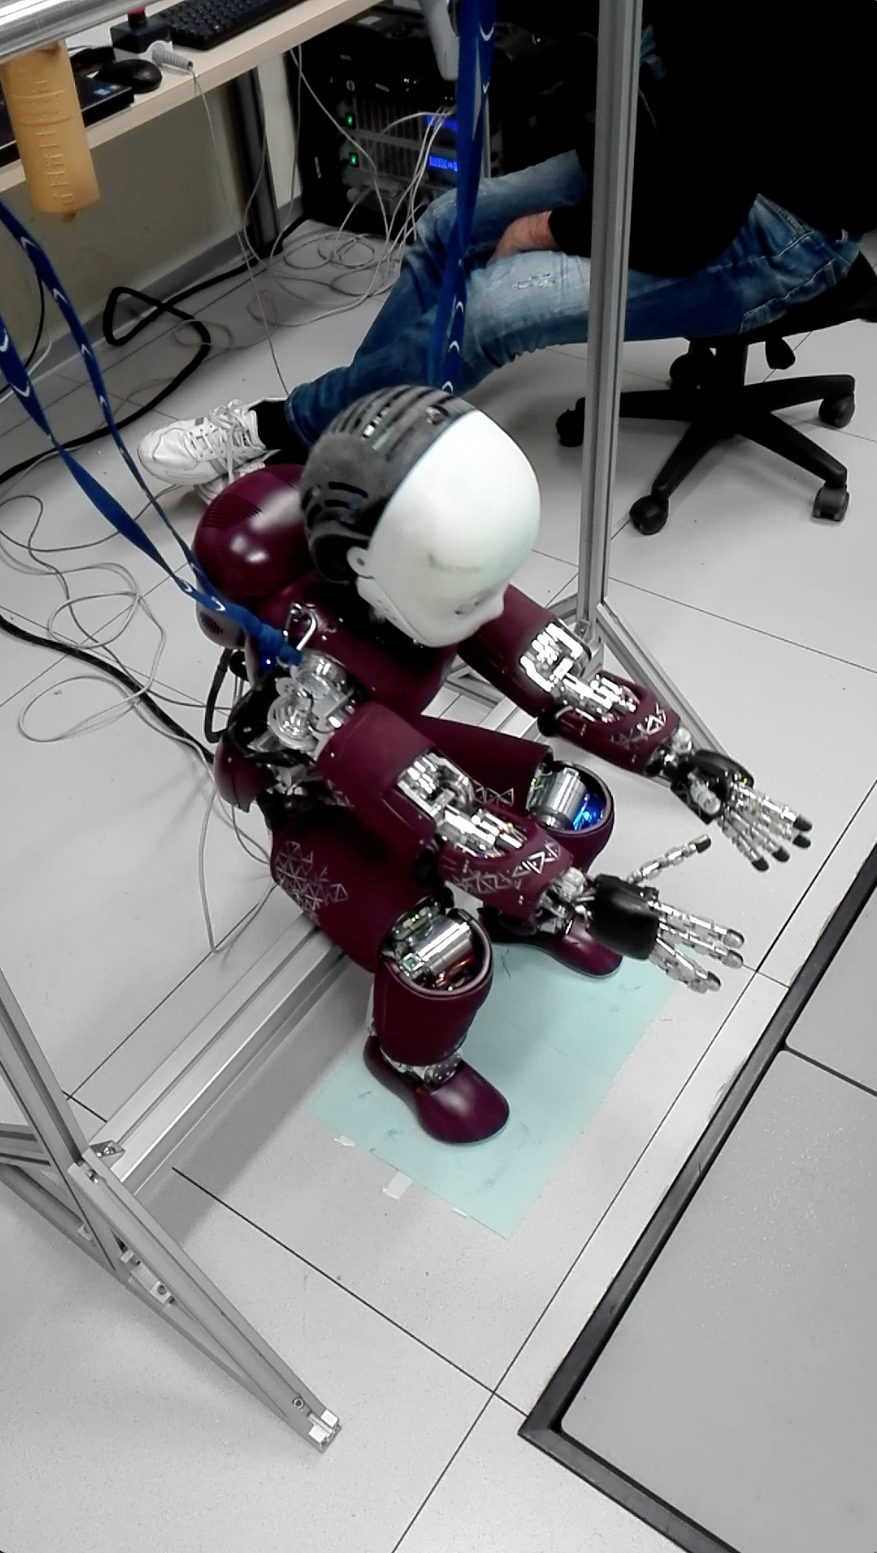
\includegraphics[width=0.25\columnwidth]{figs/standing_1} \hspace{1cm}
    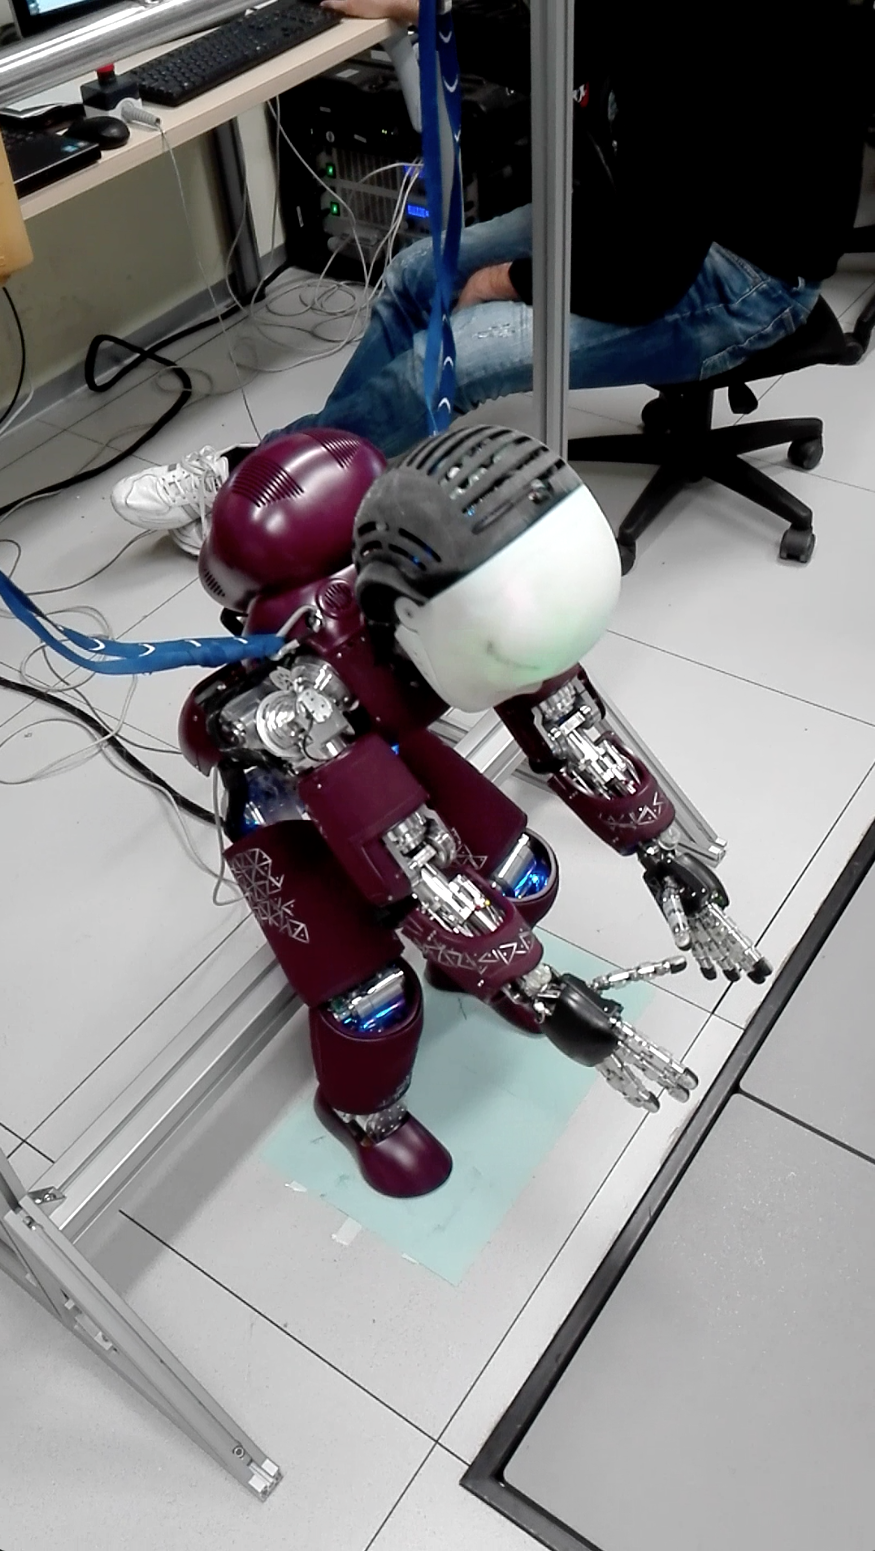
\includegraphics[width=0.25\columnwidth]{figs/standing_2} \hspace{1cm}
    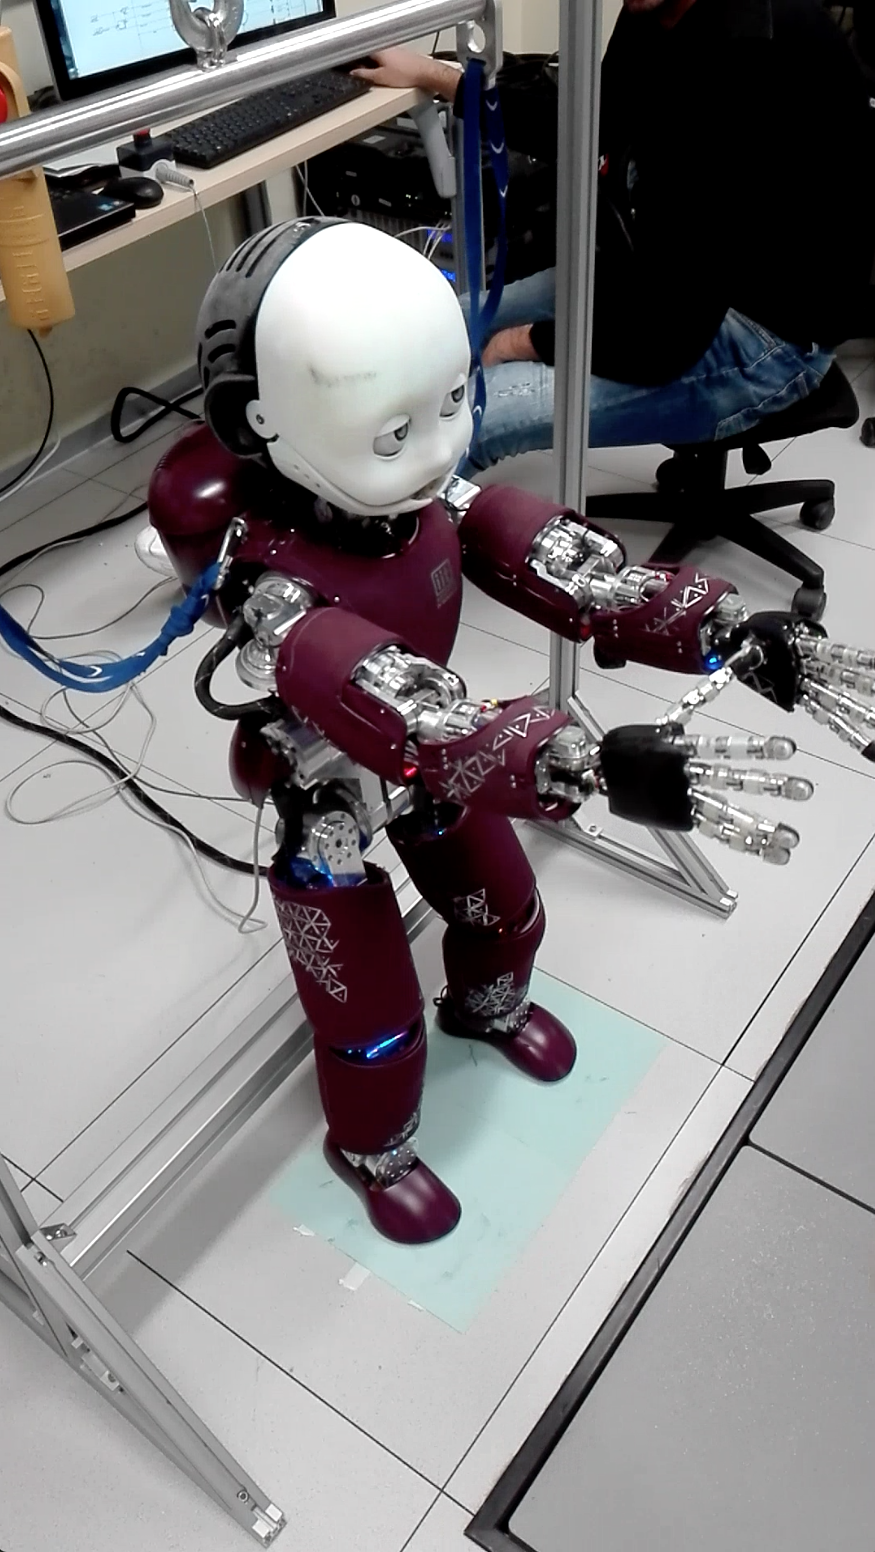
\includegraphics[width=0.25\columnwidth]{figs/standing_3}
  \caption{The iCub standing motion without external support from a caregiver. }
  \label{fig:iCubStanding}
\end{figure}